\chapter{Library Design}

A major challenge which arises when one aims to develop a software package that
implements the spectral/hp element method is to implement the mathematical
structure of the method in a digestible and coherent matter. Obviously, there
are many ways to encapsulate the fundamental concepts related to the spectral/hp
element method, depending on e.g. the intended goal of the developer or the
chosen programming language. We will (without going in too much detail) give a
an overview of how we have chosen to abstract and implement spectral/hp elements
in the \nekpp library. However, we want to emphasise that this is not the
only possible choice.

Five different sublibraries, employing this characteristic pattern, are provided
in the full \nekpp library:

\begin{itemize}
\item the standard elemental region sublibrary (StdRegions library)
\item the parametric mapping sublibrary (SpatialDomains library)
\item the local elemental region sublibrary (LocalRegions library)
\item the global region sublibrary (MultiRegions library)
\item the supporting utilities sublibrary (LibUtilities library)
\end{itemize}

This structure can also be related to the formulation of a global spectral/hp
element expansion, i.e.

\begin{align*}
  u(\boldsymbol{x})=\overbrace{\sum_{e\in\mathcal{E}}\underbrace{\sum_{n\in\mathcal{N}}\phi^e_n(\boldsymbol{x})\hat{u}^e_n}_{\mbox{\scriptsize{LocalRegions
  library}}}}^{\mbox{\scriptsize{MultiRegions
  library}}}=\sum_{e\in\mathcal{E}}\underbrace{\sum_{n\in\mathcal{N}}\phi^{std}_n\overbrace{(\left[\chi^e\right]^{-1}(\boldsymbol{x}))}^{\mbox{\scriptsize{SpatialDomains
  library}}}\hat{u}^e_n}_{\mbox{\scriptsize{StdRegions library}}}
\end{align*}

A more detailed overview of the \nekpp structure, including an overview of
the most important classes per sublibrary, is depicted in the figure below.

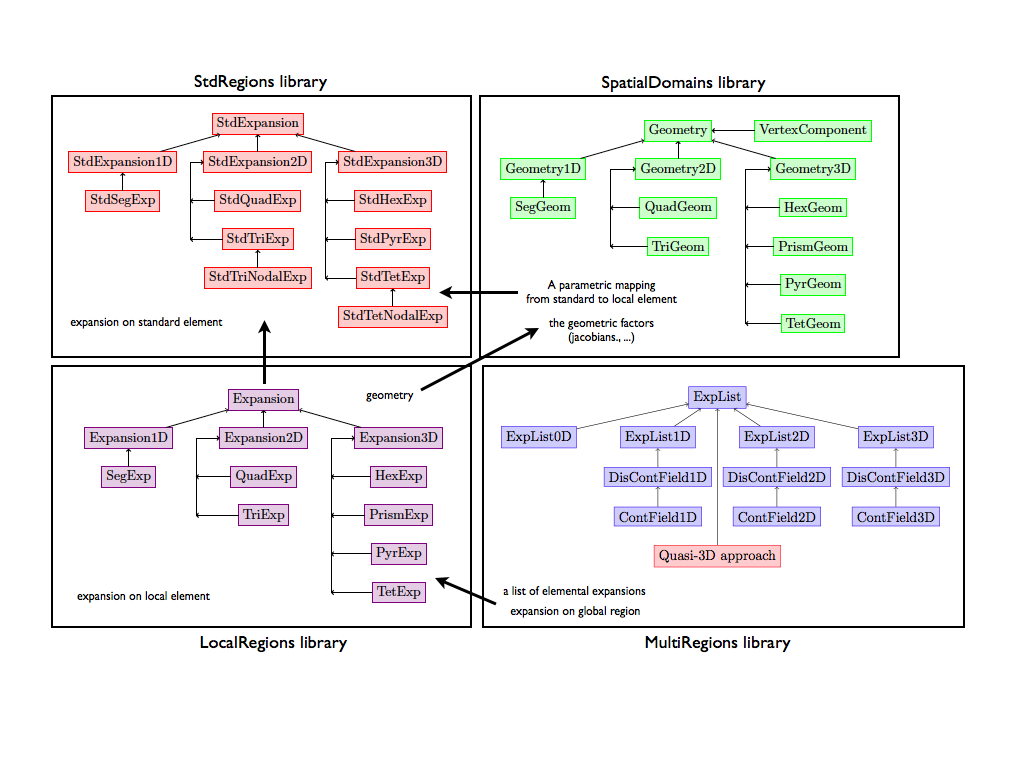
\includegraphics[width=\textwidth]{img/overview.png}

\section{LibUtilities}

This contains the underlying building blocks for constructing a Spectral Element
formulation including linear algebra, polynomial routines and memory management.

Contents
\begin{itemize}
\item Basic Constants
\item Basic Utilities ( Nektar++ Arrays)
\item Expression Templates
\item Foundations
\item Interpreter
\item Kernel
\item Linear Algebra
\item Memory Management
\item Nodal Data
\item Polynomial Subroutines
\item Time Integration
\end{itemize}

\subsection{The Polylib library}
These are routines for orthogonal polynomial calculus and interpolation based on
codes by Einar Ronquist and Ron Henderson.

\subsubsection{Abbreviations}
\begin{itemize}
\item z - Set of collocation/quadrature points
\item w - Set of quadrature weights
\item D - Derivative matrix
\item h - Lagrange Interpolant
\item I - Interpolation matrix
\item g - Gauss
\item k - Kronrod
\item gr - Gauss-Radau
\item gl - Gauss-Lobatto
\item j - Jacobi
\item m - point at minus 1 in Radau rules
\item p - point at plus 1 in Radau rules
\end{itemize}


\subsubsection{Main routines}

Points and Weights
\begin{itemize}
\item zwgj Compute Gauss-Jacobi points and weights
\item zwgrjm Compute Gauss-Radau-Jacobi points and weights (z=-1)
\item zwgrjp Compute Gauss-Radau-Jacobi points and weights (z= 1)
\item zwglj Compute Gauss-Lobatto-Jacobi points and weights
\item zwgk Compute Gauss-Kronrod-Jacobi points and weights
\item zwrk Compute Radau-Kronrod points and weights
\item zwlk Compute Lobatto-Kronrod points and weights
\item JacZeros Compute Gauss-Jacobi points and weights
\end{itemize}

Derivative Matrices
\begin{itemize}
\item Dgj Compute Gauss-Jacobi derivative matrix
\item Dgrjm Compute Gauss-Radau-Jacobi derivative matrix (z=-1)
\item Dgrjp Compute Gauss-Radau-Jacobi derivative matrix (z= 1)
\item Dglj Compute Gauss-Lobatto-Jacobi derivative matrix
\end{itemize}

Lagrange Interpolants
\begin{itemize}
\item hgj Compute Gauss-Jacobi Lagrange interpolants
\item hgrjm Compute Gauss-Radau-Jacobi Lagrange interpolants (z=-1)
\item hgrjp Compute Gauss-Radau-Jacobi Lagrange interpolants (z= 1)
\item hglj Compute Gauss-Lobatto-Jacobi Lagrange interpolants
\end{itemize}

Interpolation Operators
\begin{itemize}
\item Imgj Compute interpolation operator gj->m
\item Imgrjm Compute interpolation operator grj->m (z=-1)
\item Imgrjp Compute interpolation operator grj->m (z= 1)
\item Imglj Compute interpolation operator glj->m
\end{itemize}

Polynomial Evaluation
\begin{itemize}
\item jacobfd Returns value and derivative of Jacobi poly. at point z
\item jacobd Returns derivative of Jacobi poly. at point z (valid at z=-1,1)
\end{itemize}

\subsubsection{Local routines}
\begin{itemize}
\item jacobz Returns Jacobi polynomial zeros
\item gammaf Gamma function for integer values and halves
\item RecCoeff Calculates the recurrence coefficients for orthogonal poly
\item TriQL QL algorithm for symmetrix tridiagonal matrix
\item JKMatrix Generates the Jacobi-Kronrod matrix
\end{itemize}

\subsubsection{Useful references}
\begin{itemize}
\item `[`1`]` Gabor Szego: Orthogonal Polynomials, American Mathematical
Society, Providence, Rhode Island, 1939.
\item `[`2`]` Abramowitz \& Stegun: Handbook of Mathematical Functions, Dover,
New York, 1972.
\item `[`3`]` Canuto, Hussaini, Quarteroni \& Zang: Spectral Methods in Fluid
 Dynamics, Springer-Verlag, 1988.
\item `[`4`]` Ghizzetti \& Ossicini: Quadrature Formulae, Academic Press, 1970.
\item `[`5`]` Karniadakis \& Sherwin: Spectral/hp element methods for CFD, 1999
\end{itemize}

\subsubsection{Notes}
\begin{itemize}
\item Legendre polynomial $\alpha = \beta = 0$
\item Chebychev polynomial $\alpha = \beta = -0.5$
\item All routines are double precision.
\item All array subscripts start from zero, i.e. vector $0..N-1$
\end{itemize}

